% !TeX program = pdflatex
% =============================================================
% Public Economics -- Lecture 8
% Public Goods
% Based on: Saez, E. "Econ 131" (UC Berkeley), Lecture Notes on Public Goods
%           Gruber, J. "Public Finance and Public Policy", Ch. 7
% =============================================================
\documentclass[11pt,aspectratio=169]{beamer}

\usetheme{metropolis}
\usepackage[utf8]{inputenc}
\usepackage[T1]{fontenc}
\usepackage{lmodern}
\usepackage{booktabs}
\usepackage{array}
\usepackage{textcomp}
\usepackage{siunitx}
\usepackage{tikz}
\usepackage{pgfplots}
\pgfplotsset{compat=1.18}
\usetikzlibrary{positioning,arrows.meta,calc}
\usepackage{eso-pic}

% ----------------------------------------------------------------
% Colors: WU Vienna blue as primary accent
% ----------------------------------------------------------------
\definecolor{wublue}{HTML}{003D7C}
\definecolor{wulight}{HTML}{4F8FC4}
\definecolor{wugray}{HTML}{5C6670}
\definecolor{wured}{HTML}{B0202E}
\definecolor{wugreen}{HTML}{4C8C6B}
\definecolor{wuyellow}{HTML}{D9A441}
\setbeamercolor{palette primary}{bg=wublue,fg=white}
\setbeamercolor{frametitle}{bg=wublue,fg=white}
\setbeamercolor{progress bar}{fg=wublue,bg=wulight!30}
\setbeamercolor{alerted text}{fg=wured}

\setbeamertemplate{frame footer}{Public Goods}
\setbeamertemplate{footline}[frame number]

\title{Public Economics}
\subtitle{Lecture 8 \(\cdot\) Public Goods}
\author{Shushanik Margaryan}
\institute{WU Vienna University of Economics and Business}
\titlegraphic{
\includegraphics[height=1.0cm]{../assets/wu_logo.png}}
\date{Winter Term}

% Source note command for footnote-style citations on data slides
\newcommand{\srcnote}[1]{{\footnotesize\color{wugray}Source: #1}}

\begin{document}

% =============================================================
\begin{frame}
  \titlepage
\end{frame}

\AddToShipoutPictureFG{%
  \AtPageUpperLeft{%
    \put(\LenToUnit{\paperwidth-2.0cm},\LenToUnit{-0.85cm}){
\includegraphics[height=0.62cm]{../assets/wu_logo_white.png}}%
  }%
}

\begin{frame}{Today's Questions}
  \begin{itemize}
    \item What makes a good ``public'' in the economist's sense --- and why does the market systematically undersupply it?
    \item If everyone has an incentive to free-ride, why does \emph{any} private giving happen at all?
    \item Does government provision simply replace private giving one-for-one, or can the two coexist?
  \end{itemize}
  \vspace{1em}
  \begin{block}{Based on}
    Saez, E., \emph{Econ 131} lecture notes (UC Berkeley); Gruber, J. \emph{Public Finance and Public Policy}, Ch.\ 7.
  \end{block}
\end{frame}

% =============================================================
\begin{frame}{Outline}
  \tableofcontents
\end{frame}

% =============================================================
\section{7.1 Optimal Provision of Public Goods}

\begin{frame}{Public Goods: Definitions}
  \begin{block}{Pure public good}
    Perfectly \textbf{non-rival in consumption} and \textbf{non-excludable}.
  \end{block}
  \begin{itemize}
    \item \textbf{Non-rival:} one person's consumption doesn't reduce anyone else's opportunity to consume it.
    \item \textbf{Non-excludable:} nobody can be stopped from consuming it.
  \end{itemize}
  \begin{block}{Impure public good}
    Satisfies the two conditions only \emph{partially} --- most real-world ``public goods'' are actually this.
  \end{block}
  \vspace{0.4em}
  \small The economist's definition is narrow: it says nothing about whether a good \emph{should} be universally provided. Education and health care are not public goods in this technical sense --- they're rival and (at least partly) excludable --- even though most societies choose to provide them broadly.
\end{frame}

\begin{frame}{Recap: Optimal Provision of Private Goods}
  Two goods: ice cream ($ic$) and cookies ($c$, the num\'eraire, $P_c=1$). Two individuals, $B$ and $J$, face the same market price $P_{ic}$ but may consume different quantities.
  \begin{itemize}
    \item $MRS_{ic,c} = MU_{ic}/MU_c$ = cookies a consumer will give up for one more ice cream.
    \item \textbf{Individual optimum:} $MRS^B_{ic,c} = MRS^J_{ic,c} = P_{ic}$.
    \item \textbf{Supply-side equilibrium:} $MC_{ic} = P_{ic}$.
  \end{itemize}
  \[ \Rightarrow \quad MRS^B_{ic,c} = MRS^J_{ic,c} = MC_{ic} \]
  \small Each person separately equates their own MRS to the (common) marginal cost --- because one more ice cream for $B$ doesn't affect $J$ at all.
\end{frame}

\begin{frame}{Optimal Provision of Public Goods: The Samuelson Rule}
  Now replace ice cream with a public good --- missiles ($m$) --- consumed by \emph{both} $B$ and $J$ \textbf{simultaneously}.
  \begin{itemize}
    \item $MRS^B_{m,c}$ = cookies $B$ will give up for one more missile; $MRS^J_{m,c}$ likewise for $J$.
    \item Since both enjoy the same missile, society is willing to give up $MRS^B_{m,c} + MRS^J_{m,c}$ cookies for it.
  \end{itemize}
  \begin{block}{Samuelson Rule (Samuelson, 1954)}
    \[ MRS^B_{m,c} + MRS^J_{m,c} = MC_m \]
  \end{block}
  \small Efficiency requires marginal cost to equal the \textbf{sum} of everyone's MRS --- not each person's MRS separately, as with a private good.
\end{frame}

% =============================================================
\section{7.2 Private Provision of Public Goods}

\begin{frame}{Private-Sector Underprovision}
  Left to itself, each individual $i$ contributes only up to the point where \emph{their own} $MRS^i_{m,c} = MC_m$ --- ignoring the benefit to everyone else.
  \[ \sum_i MRS^i_{m,c} > MC_m \quad\Rightarrow\quad \text{too little of the public good is provided.} \]
  \begin{block}{Free-rider problem}
    When an investment has a personal cost but a common benefit, selfish individuals will underinvest.
  \end{block}
  \small Conceptually: private provision of a public good creates a \textbf{positive externality} on everyone else --- and, exactly as with any positive externality, the market undersupplies it.
\end{frame}

\begin{frame}{Government Provision of Public Goods}
  Providing public goods is the oldest function of government. The largest public goods are supplied almost entirely by the state:
  \begin{enumerate}
    \item National defense.
    \item Police and justice.
    \item Transportation, energy, and sanitation infrastructure.
    \item Increasingly: environmental protection.
  \end{enumerate}
  \vspace{0.3em}
  \small Basic science is typically government-funded, while applied R\&D is mostly private; a technology becomes a genuine public good once it falls into the public domain.
\end{frame}

\begin{frame}{A Formal Model of Free-Riding}
  Two identical individuals share a private good $X$ (cookies) and jointly fund a public good $F$ (fireworks), $F = F_1 + F_2$.
  \[ U_i = 2\log(X_i) + \log(F_1+F_2), \qquad X_i + F_i = 100 \]
  Individual 1 maximizes $2\log(100-F_1) + \log(F_1+F_2)$ taking $F_2$ as given:
  \[ -\frac{2}{100-F_1} + \frac{1}{F_1+F_2} = 0 \quad\Rightarrow\quad F_1 = \frac{100-2F_2}{3} \]
  \small This is individual 1's \textbf{reaction curve}: $F_1$ falls as $F_2$ rises --- the free-rider effect in action. By symmetry, $F_2 = (100-2F_1)/3$.
\end{frame}

\begin{frame}{Diagram: Reaction Curves and the Nash Equilibrium}
  \begin{center}
  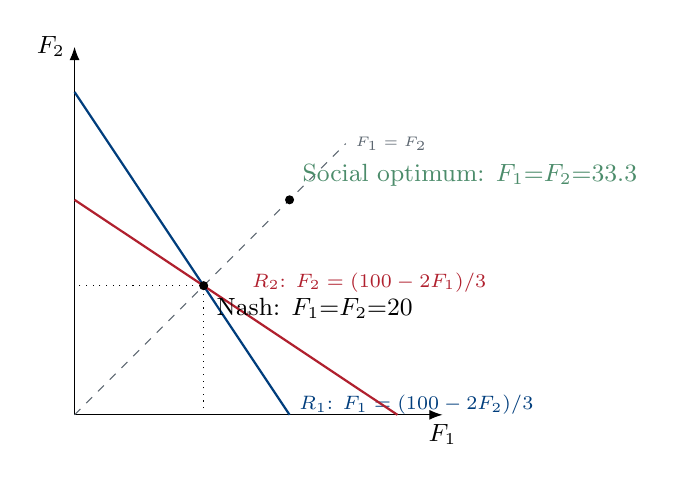
\begin{tikzpicture}[scale=0.82]
    \draw[-{Latex}] (0,0) -- (5.7,0) node[below, font=\small]{$F_1$};
    \draw[-{Latex}] (0,0) -- (0,5.7) node[left, font=\small]{$F_2$};
    \draw[wugray, dashed] (0,0) -- (4.2,4.2);
    \node[right, font=\tiny, wugray] at (4.2,4.2) {$F_1=F_2$};
    \draw[wublue, thick] (0,5) -- (3.33,0);
    \node[right, font=\scriptsize, wublue] at (3.33,0.15) {$R_1$: $F_1=(100-2F_2)/3$};
    \draw[wured, thick] (0,3.33) -- (5,0);
    \node[above right, font=\scriptsize, wured] at (2.6,1.75) {$R_2$: $F_2=(100-2F_1)/3$};
    \fill (2,2) circle (2pt); \node[below right, font=\small] at (2.05,1.95) {Nash: $F_1{=}F_2{=}20$};
    \fill (3.33,3.33) circle (2pt); \node[above right, font=\small, wugreen] at (3.38,3.38) {Social optimum: $F_1{=}F_2{=}33.3$};
    \draw[dotted] (2,0) -- (2,2) -- (0,2);
  \end{tikzpicture}
  \end{center}
  \footnotesize The two reaction curves cross at the Nash equilibrium, well \emph{below} the socially optimal contribution on the $F_1{=}F_2$ line.
\end{frame}

\begin{frame}{Nash Equilibrium vs.\ the Social Optimum}
  At the Nash equilibrium, both reaction curves hold simultaneously:
  \[ F_1+F_2 = \frac{200-2(F_1+F_2)}{3} \;\Rightarrow\; F = F_1+F_2 = \frac{200}{5} = 40 \;\Rightarrow\; F_1=F_2=20 \]
  The social optimum requires $\sum_i MRS^i = MC = 1$, with $MRS^i_{F,X} = \dfrac{X_i}{2F}$:
  \[ \sum_i MRS^i = \frac{200-F}{2F} = 1 \;\Rightarrow\; F = \frac{200}{3} = 66.6 \; > \; 40 \]
  \begin{alertblock}{Public goods are under-provided by the market}
    Free-riding cuts total fireworks nearly in half relative to the efficient level.
  \end{alertblock}
\end{frame}

\begin{frame}{In-Class Game: A Public Goods Experiment}
  \begin{block}{Setup}
    You're in a group of 5. You have 10 tokens. 1 token kept privately $=$ \$1 for you. 1 token given to the group $=$ \$0.50 to \emph{each} of the 5 members (including you) --- \$2.50 total.
  \end{block}
  How would you split your 10 tokens?
  \begin{enumerate}
    \item[A.] All 10 to the private good.
    \item[B.] All 10 to the public good.
    \item[C.] Split them half and half.
  \end{enumerate}
  \vspace{0.4em}
  \small Nash equilibrium (selfish play): keep everything privately. Socially optimal: contribute everything --- \$1 kept is worth less to the group than \$2.50 shared.
\end{frame}

\begin{frame}{Experimental Evidence on Free-Riding}
  \textbf{Marwell \& Ames (1981):} 10 repetitions of the game above (group of 5, 10 tokens each; private return \$1, public return \$0.50 to each of 5).
  \begin{itemize}
    \item \textbf{Nash prediction:} contribute nothing.
    \item \textbf{Social optimum:} contribute everything.
    \item \textbf{What actually happens:} subjects contribute roughly \textbf{50\%} to the public good.
  \end{itemize}
  \vspace{0.4em}
  \textbf{Isaac, McCue \& Plott (1985):} contributions \textbf{decline} the more the game is repeated --- people start out willing to cooperate, then get upset and retaliate once they see others taking advantage.\\
  \srcnote{Marwell \& Ames (1981); Isaac, McCue \& Plott (1985).}
\end{frame}

\begin{frame}{Why Do People Cooperate?}
  In the standard model, selfish individuals play Nash and free-ride. Yet humans plainly cooperate constantly --- in families, workplaces, communities, nations.
  \begin{itemize}
    \item Cooperation appears to be \textbf{innate}, sustained by a sense of fairness and a willingness to \textbf{punish non-cooperators} even at a cost to the punisher (``altruistic punishment'').
    \item Likely an evolutionary adaptation.
    \item Fehr \& Schmidt (1999) formalize ``fairness preferences'' in a large lab literature.
  \end{itemize}
  \vspace{0.4em}
  \small These social motives are still only partially integrated into mainstream economic models --- a real limitation, especially for public economics.
\end{frame}

% =============================================================
\section{7.3 Crowding Out and Government Provision}

\begin{frame}{Crowding Out: A Formal Model}
  Suppose government now \textbf{forces} each individual to contribute 5, so $F = F_1+F_2+10$, where $F_i$ is now \emph{voluntary} top-up:
  \[ U_i = 2\log(X_i) + \log(F_1+F_2+10), \qquad X_i+F_i = 95 \]
  Solving gives $F_1=F_2=15$ --- \textbf{one-for-one crowd-out} of the forced contribution.
  \begin{itemize}
    \item \textbf{Why?} Let $F_i' = F_i+5$. Then $U_i=2\log(X_i)+\log(F_1'+F_2')$ with $X_i+F_i'=100$ --- \emph{identical} to the original (no-government) problem, so $F_i'$ must be the same: $F_i'=20 \Rightarrow F_i=15$.
    \item Crowd-out stops being one-for-one only once voluntary contributions hit \textbf{zero} --- you can't ``un-contribute'' a negative amount.
  \end{itemize}
\end{frame}

\begin{frame}{Empirical Evidence on Crowd-Out}
  \begin{block}{Crowd-out}
    The reduction in private contributions caused by an increase in government provision of the same public good.
  \end{block}
  Two strands of evidence:
  \begin{enumerate}
    \item \textbf{Field evidence} (observational studies).
    \item \textbf{Lab and field experiments.}
  \end{enumerate}
  \vspace{0.4em}
  \small Lab experiments (Andreoni, 1993) find crowd-out is real but \textbf{imperfect} --- well below the one-for-one prediction of the simple model. Lab settings likely miss important real-world motives for giving: warm glow, prestige, and active solicitation by fundraisers.
\end{frame}

\begin{frame}{Charitable Giving in Practice}
  Charitable giving is one form of private public-good provision.
  \begin{itemize}
    \item In the US, giving totals about \textbf{1.5\% of national income} --- large in absolute terms, but far smaller than the gap in government spending between the US ($\approx$30\% of national income) and the EU ($\approx$45\%).
    \item Funds flow mainly to: religious organizations, education, human services, health, the arts, and other causes (environment, etc.).
    \item Governments actively \textbf{encourage} it: charitable gifts are typically deductible from taxable income.
  \end{itemize}
\end{frame}

\begin{frame}{Why Do People Give?}
  \begin{enumerate}
    \item \textbf{Warm glow} --- e.g., your name on a building.
    \item \textbf{Reciprocity} --- e.g., alumni giving back to their university.
    \item \textbf{Social pressure} --- e.g., giving at church, in front of others.
    \item \textbf{Altruism} --- e.g., poverty relief for its own sake.
  \end{enumerate}
  \vspace{0.5em}
  \small None of these motives are captured by the basic free-rider model above --- which is exactly why charities run large fundraising operations built around social and psychological cues, not just the pure economics of public-good provision.
\end{frame}

\begin{frame}{Evidence: Andreoni \& Payne (2003) on Crowd-Out}
  Government spending can crowd out private donations through \textbf{two} channels: reduced willingness to give, \emph{and} reduced fundraising effort.
  \begin{itemize}
    \item Panel data on arts and social-service organizations' tax returns, followed over time.
    \item \textbf{Finding:} a \$1{,}000 increase in a government grant leads to about \$250 less private fundraising.
  \end{itemize}
  \small Most of the crowd-out operates through the \textbf{fundraising} channel: less government funding means organizations fundraise harder (e.g., federal funding cuts to universities tend to boost their own fundraising drives).
  \vspace{0.4em}
  \begin{alertblock}{Crowding \emph{in}}
    Kotchen \& Wagner (2023): when the US spends more on national parks, \textbf{volunteer hours rise too} --- government spending can crowd private effort \emph{in}, not just out.
  \end{alertblock}
\end{frame}

\begin{frame}{Field Experiment: Reciprocity in Giving}
  \textbf{Falk (2007):} 10{,}000 Christmas solicitation letters (funding schools for street children in Bangladesh) sent to Swiss donors, randomized into three groups.
  \begin{center}
  \begin{tabular}{@{}lcc@{}}
    \toprule
    \textbf{Group} & \textbf{Gift included} & \textbf{Response rate} \\
    \midrule
    Control & None & 12\% \\
    Treatment 1 & Small (1 postcard + envelope) & 14\% \\
    Treatment 2 & Large (4 postcards + envelopes) & 21\% \\
    \bottomrule
  \end{tabular}
  \end{center}
  \vspace{0.4em}
  \small A larger upfront gift substantially raised giving --- consistent with reciprocity, and effective even relative to its cost.\\
  \srcnote{Falk (2007), \emph{Econometrica} 75(5).}
\end{frame}

\begin{frame}{Field Experiment: Social Pressure in Door-to-Door Giving}
  \textbf{DellaVigna, List \& Malmendier (2012):} a randomized door-to-door fundraiser experiment.
  \begin{itemize}
    \item \textbf{Control:} no advance warning of the visit.
    \item \textbf{Treatment 1:} a doorknob flyer announces the exact visit time (so residents can seek out --- or avoid --- the fundraiser).
    \item \textbf{Treatment 2:} same flyer, plus a ``Do not disturb'' checkbox.
  \end{itemize}
  \textbf{Results (vs.\ control):} Treatment 1 --- 9--25\% less likely to open the door, unconditional giving unchanged. Treatment 2 --- many opt out, and unconditional giving falls 28--42\%.
  \vspace{0.3em}
  \small Social pressure is a real determinant of door-to-door giving --- and the fundraiser's visit itself \emph{lowers} the utility of potential donors.
\end{frame}

\begin{frame}{Social Prices as a Policy Instrument}
  Beyond taxes and subsidies, policy can try to shift \textbf{social norms} directly --- ``social prices.''
  \begin{itemize}
    \item Make a positive-externality behavior a status symbol: electric cars are increasingly admired, while large gas-guzzling SUVs are increasingly frowned upon (Butera et al., 2022).
    \item Social-price elasticities can be large: Gerber, Green \& Larimer (2008) show that a letter using social pressure (``your neighbors will see whether you voted'') substantially raises voter turnout.
  \end{itemize}
\end{frame}

\begin{frame}{Welfare Analysis of Social Pricing}
  Should social pricing be layered \emph{on top of} standard corrective taxes or tradable permits?
  \begin{itemize}
    \item \textbf{Shaming SUV drivers} is generally \textbf{inefficient} relative to a gas tax: it destroys welfare without raising any revenue. It can still be worthwhile when a fine or tax is hard to enforce at all --- e.g., social disapproval of littering, where fines are difficult to levy.
    \item \textbf{Praising efficient-car owners}, by contrast, is \textbf{efficient} relative to a gas tax: it adds to welfare, since driving the energy-efficient car becomes more enjoyable in itself.
  \end{itemize}
\end{frame}

% =============================================================
\begin{frame}{Sources}
  \tiny
  \begin{columns}[T]
    \begin{column}{0.34\textwidth}
      Andreoni, J. (1993), \emph{AER}.\\
      Andreoni, J. \& Payne, A. (2003), \emph{AER}.\\
      Butera et al. (2022), \emph{AER} 112(1).\\
      DellaVigna, List \& Malmendier (2012), \emph{QJE} 127(1).
    \end{column}
    \begin{column}{0.34\textwidth}
      Falk, A. (2007), \emph{Econometrica} 75(5).\\
      Fehr \& Schmidt (1999), \emph{QJE} 114(3).\\
      Gerber, Green \& Larimer (2008), \emph{APSR} 102(1).\\
      Gruber, J., \emph{Public Finance and Public Policy}, Ch.\ 7.
    \end{column}
    \begin{column}{0.34\textwidth}
      Isaac, McCue \& Plott (1985), \emph{JPubE} 26(1).\\
      Kotchen \& Wagner (2023), \emph{JPubE} 222.\\
      Marwell \& Ames (1981), \emph{JPubE} 15(3).\\
      Saez, E., \emph{Econ 131} lecture notes, UC Berkeley.\\
      Samuelson, P. (1954), \emph{REStat} 36(4).
    \end{column}
  \end{columns}
\end{frame}

\begin{frame}[standout]
  Thank you!\\
  \vspace{0.5em}
  \small Questions and discussion
\end{frame}

\end{document}
